\frame{
\begin{center}
{\Large Differential equations} are commonly used for mathematical modeling in science and engineering.  \\
\vspace{0.5cm}
Often, there is no known analytic solution and numerical approximations are required. 
\end{center}
}



\frame{
\begin{block}{The Lotka- Volterra equations : }
\begin{equation*}
\begin{array}{r l}
x′ & = f(t,x,y)=x-xy- \frac{1}{10} x^2 \\
& \\
y′ & =g(t,x,y)=xy-y- \frac{1}{20} y^2,
\end{array}
\end{equation*}
with the initial condition $x(0) = 2$ and $y(0) = 1$ for $0 \le t \le 30$.
\end{block}
%\begin{figure}
%\begin{center}
%\includegraphics[width=100mm]{fig/ch-6/p_245.png}
%\end{center}
%\end{figure}
Although the numerical solution is a list of numbers, it is helpful to plot the polygonal path joining the approximation points $\{( x_k, y_k)\}$ and plot the trajectory shown in the following figure\footnote{Figure 6.1}. 
\begin{figure}
\begin{center}
%\includegraphics[width=100mm]{fig/ch-6/fig_6-1.png}
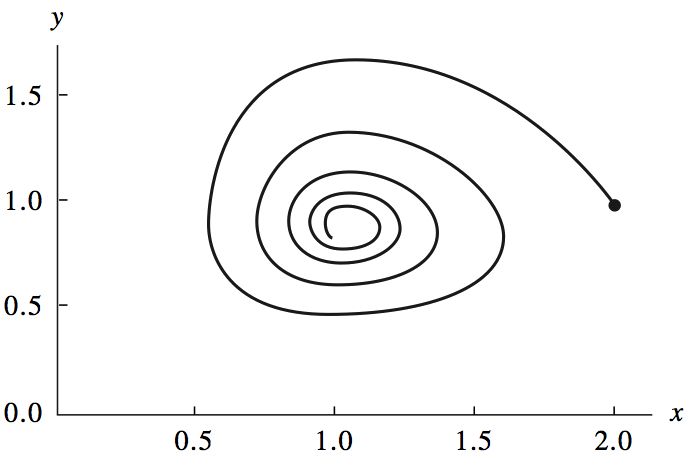
\includegraphics[width=50mm]{chap-6/fig_9-1.png}
\end{center}
\end{figure}
}



\frame{
\begin{block}{}
\begin{center}
In this chapter we present the standard methods for solving { \huge ordinary differential equations}, {\huge systems of differential equations}, and {\Huge boundary value problems}. 
\end{center}
\end{block}
}